%%% NEW IMPLEMENTATION
\chapter{New implementation}\label{c:new_impl}

In this chapter we present the main contribution of this thesis: the new and improved implementation of the model. First, we provide an overview of the program and the design philosophy behind it. Then, we go over the features of the reference implementation and discuss how they are implemented in the new program. Finally, we present performance optimizations that we have developed in addition to the already present ones.

\section{Design}\label{new:design}

Reference implementation provides the means of simulating a number of altogether separate scenarios, which are nevertheless joined together in the form of a single program. These share a common foundation in the form of file parsers, forces and other ancillary features. It is natural to extract this foundation into a library of components which the users can freely use to construct their own scenarios. Our efforts focused on developing a system of abstractions, which would govern the structure of this library and would allow users to develop their particular simulation scenarios without having to know the ins and outs of the implementation, as well as let them easily create new components. We have arrived at a following set of design choices:

\begin{enumerate}
    \item There should be a ``centerpiece'' class which represents the entire simulation. We also considered the alternative of providing all the components separately and letting users link them, as though they were essentially functions, however we felt that this kind of code would become burdensome to write and not provide any benefits to the end user.
    \item One should be able to instantiate it with ease, using objects representing the initial state and the parameters of the simulation generated by an array of provided file parsers.
    \item The simulation object should provide a way to add various objects representing forces that act on the pseudoatoms, as well as any other computations that should happen during a simulation step. These objects should be independent of each other as much as possible.
    \item Performing a simulation step should be straightforward, preferably a single function call, as opposed to a number of function calls spread out in the code in multiple places.
    \item Implementation details should be hidden from the user.
\end{enumerate}

With these changes, the intricate user interface of the original program has been replaced with a more declarative one which should better convey the structure of the simulation scenario in question. Listing \ref{list:new_prog} shows an example of a simulation scenario composed of different library components:

\begin{lstlisting}[language=C++,caption=Example scenario that simulates an ordered protein]
int main() {
    ifstream param_file("data/parametersMJ96.txt");
    auto params = param::LegacyParser().read(param_file);
    
    ifstream pdb_file("data/1ubq.pdb");
    auto atomic = pdb::Parser().read(pdb_file).asModel();
    atomic.addContactsFromAtomOverlap();
    auto model = atomic.coarsen();

    Random rand(448);
    // Initial conditions
    model.morphIntoSAW(rand, false, 0.0, 4.56*angstrom, true);
    model.initVelocity(rand, 0.35 * eps_kB, false);

    Simulation simul(model, params);

    simul.add<Random>(rand);
    
    // Add the integrator 
    simul.add<LangPredictorCorrector>(0.005 * tau);

    // Add forces
    simul.add<Tether>(true);
    simul.add<NativeBA>();
    simul.add<ComplexNativeDihedral>();
    simul.add<NativeContacts>();
    simul.add<PauliExclusion>();

    // Add hooks
    auto total = 15000.0*tau;
    simul.add<ProgressBar>(total, 10.0*tau);
    simul.add<ExportPDB>("result.pdb", 100.0*tau);

    // Run the simulation
    simul.step(total);
    return 0;
}
\end{lstlisting}\label{list:new_prog}


It should be quite clear how an end user of the library can load the requisite resources, operate on them, instantiate a simulation object with them, choose an integrator, add force fields and additional actions to perform and finally run the simulation. In contrast, constructing similar scenario in the original program would require setting appropriate global variables and by extension understanding the semantics and interactions of all provided settings of the program. Adding a new scenario would require adding these options manually to the list of global variables, as well as having to modify potentially unrelated code in order to accommodate the addition, potentially breaking it.

We will now elaborate on the implementation details of this system.

\subsection{\texttt{Simulation} class}
\texttt{Simulation} class is the centerpiece of the library: it provides a declarative interface for preparing and running the simulation and hides the implementation details from users. For an end user, two methods are available.

The method \texttt{step(double t)} performs a number of simulation steps, i.e. computes forces (see subsection \ref{new:impl_model} for details), runs hooks, integrates the equations of motion and advances the internal clock by $\Delta t$ until the total of $t$ time has passed.

The method \texttt{add<T>(x1, ..., xn)} is more involved. It adds an object \texttt{T(x1, ..., xn)} to the simulation. We wanted to achieve a uniform interface, so this method does different things depending on the type \texttt{T}. If it is a force, we add it to the list of forces. If it is an integrator, we replace the current integrator with it. This is internally achieved by using a heterogeneous collection. The implementation also automatically manages memory. Although in the original implementation the memory management was not an issue, this was rather due to it being statically allocated, which created a host of other problems, such as possible overflows or excessive memory usage of the program.

Objects added to the simulation may require access to other objects present in the same simulation. For example, non-local forces naturally require access to the Verlet list and all forces need access to \texttt{State}, which holds pseudoatoms' positions. This is handled by two mechanisms:

\begin{enumerate}
    \item Objects may inherit an interface \texttt{SimulVar} with a method \texttt{bind(Simulation\&)}, which completes the initialization of an object when it is added to a simulation.
    \item Method \texttt{simul.var<T>()} allows any object to obtain a reference to the object of type \texttt{T} added to the simulation. If such an object does not exist yet, it will be constructed and added. Thanks to this setup, the user of the library does not have to manually add objects that are used internally by forces and hooks. For example, it is not necessary to explicitly add the Verlet list, the first non-local force will add it automatically.
\end{enumerate}

We also prevent adding or accessing simulation variables after the simulation has started. This has the effect of requiring component developers to fetch all the necessary dependencies during the binding phase. So understanding all the inter-component dependencies requires only reading the implementations of the \texttt{bind} methods.

The final interface is type- and memory-safe, concise, hides implementation details and yet is extensible.

\subsection{I/O and model preparation}
Before the simulation can be started, one needs to prepare the state, which includes initial positions and velocities of the amino acids. It is also necessary to prepare model parameters, such as amino acid radii or various force coefficients. In the Fortran implementation, the preparation layer and the simulation layer of the program were tightly connected, in particular they operated on the same global variables and used the same data formats. We argue that they should rather be separated as much as possible. For one, their design philosophies are different: preparation layer, by virtue of being visible to the user, must be convenient to work with, whereas the simulation layer objects are hidden behind \texttt{Simulation} and are subordinated to performance considerations. Moreover, file parsers and other intermediate objects should not depend on the parts of the program which use them. In the new design, we have achieved such a separation --- the only part where the layers interact with each other are \texttt{Model} and \texttt{Parameter} classes, which represent state and the parameters of the simulation respectively, and which form an input to the \texttt{Simulation} object. We provide parsers for all files used in the original program, as well as a custom, modular parser of PDB files. It allows generating better stardards-complying and comprehensive output PDB files compared to the original implementation, which produced files that caused issues with third-party software that analyzed them. Parsers and data objects generated by them have been separated, so that new file formats can be introduced by simply writing a parser class, without having to change any other parts of the code.

\subsection{Simulation hooks}
We also provide a uniform interface for various actions that are performed after the evaluation of all force fields --- the class \texttt{Hook} with a method \texttt{void execute()}. Users can define custom classes deriving from \texttt{Hook} and add it to the \texttt{Simulation} object via \texttt{add} method, which will invoke them automatically after the integration of the equations of motion.

\section{Abstractions in the performance-critical code}\label{new:abs}
Many of the design decisions taken during the development of the reference program that resulted in inelegant code were dictated by performance considerations. Given that much of the time developing an extension to the library, in particular introducing new force fields, is spent writing performance-critical code, it was crucial to show that legibility of the code, use of abstractions and comfort of the programmer needs not be sacrificed for the speed of the simulation.

\subsection{Linear algebra}
In order to make the linear algebra code more concise and natural we used the \emph{Eigen} library \cite{eigen}. It exposes a user-friendly interface for performing calculations, utilizing the flexibility of C++ operator overloading and expression templates, which make the resulting code expand to a Fortran-equivalent during compilation. Example is provided in Figure \ref{f:dihedral}

\begin{figure}[ht]
    \noindent
    \begin{minipage}{.5\textwidth}
      \begin{lstlisting}[language={[77]Fortran}]
      ux1=rx(2)-rx(1)
      uy1=ry(2)-ry(1)
      uz1=rz(2)-rz(1)
    
      ux2=rx(3)-rx(2)
      uy2=ry(3)-ry(2)
      uz2=rz(3)-rz(2)
    
      ux3=rx(4)-rx(3)
      uy3=ry(4)-ry(3)
      uz3=rz(4)-rz(3)
    
      vx1=uy1*uz2-uz1*uy2
      vy1=uz1*ux2-ux1*uz2
      vz1=ux1*uy2-uy1*ux2
      vv1=vx1*vx1+vy1*vy1+vz1*vz1
    
      vx2=uy2*uz3-uz2*uy3
      vy2=uz2*ux3-ux2*uz3
      vz2=ux2*uy3-uy2*ux3
      vv2=vx2*vx2+vy2*vy2+vz2*vz2
    
      v12=vx1*vx2+vy1*vy2+vz1*vz2
      v12=v12/sqrt(vv1*vv2)
      v12=min(v12,1.d0)
      v12=max(v12,-1.d0)
      phi=dacos(v12)
    
      di=vx1*ux3+vy1*uy3+vz1*uz3
      if(di.lt.0.d0) phi=-phi
      \end{lstlisting}
    \end{minipage}%
    \begin{minipage}{.5\textwidth}
      \begin{lstlisting}[language=C++]
      Vector u1 = r2 - r1;
      Vector u2 = r3 - r2;
      Vector u3 = r4 - r3;
      
      Vector v1 = u1.cross(u2);
      Vector v2 = u2.cross(u3);
      
      double cos_phi = v1.dot(v2) / sqrt(v1.squaredNorm() * v2.squaredNorm());
      
      cos_phi = max(min(cos_phi, 1.0), -1.0);
      double phi = acos(cos_phi);
      if (v1.dot(u3) < 0.0) phi = -phi;
      \end{lstlisting}
    \end{minipage}
    \caption{Comparison of Fortran (left) and C++ (right) implementations for the computation of dihedral angle between four consecutive pseudoatoms. The C++ version is much shorter and better conveys the intent behind the function.}
    \label{f:dihedral}
\end{figure}


\subsection{Force kernels}
Many of the force fields present in the model use the Lennard-Jones potential \cite{lj} with varying potential depths and values of the minimum radius. In the Fortran code, these parameters are global, and the code computing the forces acting on each residue and the potential energy is replicated every time, sometimes in a slightly modified form. We recognized this as an opportunity to extract it and similar constructs into \emph{force kernels}, which hold the parameters necessary for computing forces and potential energy. By implementing the computations of the potential energy and forces as inlined functions as opposed to placing them in \texttt{*.cpp} file, the function call overhead is not incurred. Because the parameters for the evaluation are now in one place, one needs to know less of other parts of the code. Finally, it allows us to implement more complex force fields in a more elegant fashion, by storing many such kernels in the force field class and invoking the force/energy computation forces as required.

\subsection{Physical units}
Physics simulations require storing various physical quantities, such as forces, energies and distances. They are usually represented in internal units as opposed to SI. In the Fortran version, this aspect of the implementation was handled in an inadequate fashion. Most inputs were assumed to be in the internal units, except for the distance values read from PDB files and certain config parameters, which were scaled. This kind of approach is inflexible, as in order to change the internal units one would have to change many of the input files and simulation parameters. It is also difficult to convert standard units to the internal units and back, because some of internal units are not explicitly assigned values in terms of SI units. One can easily introduce errors by forgetting what the proper units of a particular quantity are. In fact, we have found one such bug in the original code.

We resolved all these issues by having a single file \texttt{Units.hpp} with all the units, and specifying all the physical quantities present in the code with the appropriate unit. Now, changing the units of the simulation requires changing values in a single file, and it is harder to introduce bugs. We also define all SI units, which makes the conversion between internal and standard units easy.

\section{Features}\label{new:features}

In this section we go through some of the features of the reference program and briefly discuss how they are implemented in the new program.

\subsection{Verlet list}

In contrast with the reference program, Verlet list is completely free of potentials' implementation details. It has a simple interface. Objects of class \texttt{NonlocalForce} specify what is their required cutoff distance and provide their implementation of \texttt{vlUpdateHook}, which is a function that will be called each time the list is updated. The list holds only pairs of indices pointing to two pseudoatoms that may be closer than the cutoff. If some potential needs to keep some data for each pair in the list, it needs to maintain it itself, usually by updating its internal list in the \texttt{vlUpdateHook}. This greatly simplifies Verlet list's implementation and the clear interface increases readability. Additionally, we have implemented significant optimizations for updating the list, which we describe in subsection \ref{opt:verlet}.

\subsection{Simulation protocols}

Each simulation protocol translates to a subset of objects added to the \texttt{Simulation} object. If one needs wall interactions, one should add the relevant potential to the simulation. If one wants the simulation to end once all native contacts are present, it can be achieved by using a simple \texttt{Hook}, which holds a reference to \texttt{NativeContacts} object and after each step it checks the number of present native contacts. This design makes it easy to see what particular simulation is supposed to do by just looking at the code that builds the \texttt{Simulation} object.

\subsection{Boundary conditions}

Wall interactions are implemented using \texttt{Force} interface, just like all other potentials. A small \texttt{Topology} class deals with concerns surrounding the simulation box. It provides current positions of the box's walls and can calculate the shortest vector between two points in space, which matters only if the periodic boundary conditions are enabled.

\subsection{Checkpoints}

Saving and loading a checkpoint requires being able to save and load the internal state of all objects added to the simulation. The internal state can be defined as the data that can change in one step and then be used in another step. Most notable examples include pseudoatoms' positions and their derivatives, adiabatic counters used in quasi-adiabatic potential and dimensions of the simulation box. Verlet list also satisfies this definition, because we reuse it between steps for performance reasons, but it is not necessary to save it, since it can always be rebuilt from other data. 

We extended \texttt{SimulVar} interface with two methods: \texttt{serialize} and \texttt{deserialize}, which respectively save and load internal state using a human-readable format. This allows us to easily serialize and deserialize the whole simulation object using polymorphism.

\section{Parallel processing}\label{new:parallel}

Both reference and new implementation use the OpenMP~\cite{openmp} library. It provides compiler directives and environmental variables that form a high-level API for portable shared memory parallelism. Its biggest advantage is its simplicity. If the user wants to run a loop in parallel, all it takes is to write one short directive above and the compiler will automatically insert code that prepares a thread pool, distributes loop iterations between threads and joins them after. 

The reference implementation used OpenMP to parallelize loops that are responsible for most of the computations i.e. calculating forces and integrating the equations of motion. Each loop is parallelized individually, which generates many unnecessary synchronization barriers, slowing down the simulation.
Another issue is that the authors did not protect shared data, which resulted in multiple race conditions. One could avoid those by using atomic instructions and proper synchronization techniques, but even then the original design would suffer from non-determinism, because there are some potentials where creation of one contact prohibits the creation of another. 

We decided to also use OpenMP for the new implementation, because it is portable, simple and familiar to the future users. However, instead of  handling each force individually, we used it to implement a simple abstract model of computation that is restrictive enough to be easily parallelizable, thread-safe and deterministic, while powerful enough to enable implementing all forces in a way that efficiently makes use of multiple threads. 

\subsection{Model of computation}

All forces must implement the \texttt{Force} interface. It requires implementing two methods: \texttt{asyncPart} and \texttt{syncPart}, both return \texttt{void} and take one argument --- a reference to an object of class \texttt{Dynamics}. It holds intermediate results of force computations, namely the total potential energy and the total force vector for each pseudoatom. All it takes to compute a single force is to first call its \texttt{asyncPart} and then its \texttt{syncPart}. The result will be added to the provided \texttt{Dynamics} object. These two methods have different semantics and their implementations must adhere to different rules:

\begin{itemize}
    \item \texttt{asyncPart}: This method is called in a multi-threaded setting. Data that is accessed in \texttt{asyncPart} by more than one \texttt{Force} class must not be modified, except for the \texttt{Dynamics} object provided in the argument. The entire body of this function should consist of one or more \texttt{for} loops, each prepended with \texttt{omp-for} directive.
    
    \item \texttt{syncPart}: This method is called in a single-threaded setting and it is guaranteed that it will be called after all other \texttt{asyncPart} computations finished. When there are many forces in the simulation, their \texttt{syncPart}s will be called in the order in which they were added to the simulation, so this order is fully controlled by the user. There are no limitations on the implementation, but obviously for efficiency it must be kept as fast as possible. 
\end{itemize}


The general idea is simple. As much of the computations as possible should be in \texttt{asyncPart}, but this method is much more constrained. Still, most of the potentials can be implemented without using \texttt{syncPart} at all. Most notably, all the potentials that are \emph{functional} in nature, meaning that they do not have any internal state and do not modify any data outside of the \texttt{Dynamics} object. 

\subsection{Implementing the model}\label{new:impl_model}

Calculating the forces using the interface above is straightforward when using OpenMP. The only interesting thing is ensuring that the code in \texttt{asyncPart} can freely modify the \texttt{Dynamics} object passed as an argument. The idea is to create a separate \texttt{Dynamics} object for each thread and combine them at the end in a critical section. Creating a private copy of an object for each thread can be done easily by using \texttt{threadprivate} directive, which will handle it in a way that is invisible to the user. Usually it works by putting it in Thread Local Storage, but this is dependent on architecture and library implementation. 

The whole code that implements this model of computation is shown in Listing \ref{list:parallel}.

\begin{lstlisting}[caption=Implementation of the described computation model]
#pragma omp parallel {
    dynamics_tp.clear();
        
    for (Force* force: forces) {
        force->asyncPart(dynamics_tp);
    }
    
    #pragma omp critical {
        state.updateDynamics(dynamics_tp);
    }
}

for (Force* force: forces) {
    force->syncPart(state.dynamics);
}
\end{lstlisting}\label{list:parallel}

\subsection{Example}\label{new:example}
Here we will review a more complicated example of two forces using the model of computations described above. The \texttt{NativeContacts} potential has a fixed list of pairs that interact with each other. Every such pair has a threshold distance and whenever the pseudoatoms are closer than this threshold, we say that there is a contact between them. Another potential --- \texttt{QuasiAdiabatic} --- dynamically creates and destroys contacts between pairs of pseudoatoms and calculates forces only between pairs in contact. One of the conditions for creating a contact is that each pseudoatom has a limit on the number of contacts it can be a part of. However, this limit also includes contacts defined by \texttt{NativeContacts}. 

All of this makes it challenging to parallelize those two forces. But the experiments show that an overwhelming part of computations in \texttt{QuasiAdiabatic} is spent on checking other conditions for contact creation and computing forces. An efficient solution is to do those computations in the \texttt{asyncPart}. There we create a list of potential contacts, which satisfy all conditions except for the limit on the number of other contacts. Finally, we check the last condition in \texttt{syncPart}, where we control the order of execution, which gives us determinism. All the computations relating to \texttt{NativeContacts} are performed in its \texttt{asyncPart}. There we calculate the numbers of native contacts for each pseudoatom and those values will be ready to use once \texttt{QuasiAdiabatic}'s \texttt{syncPart} is called. 
To sum up, we did not need to use complicated synchronization techniques and achieved determinism at a cost of doing a little part of computations sequentially.   

\subsection{More parallelism}\label{new:more_parallelism}
Parallelizing force computations is the most important factor when it comes to speed, since they take the most of the time. But there are other parts of code where the program spends a non-negligible amount of time and they can quickly become bottlenecks if they do not make use of multiple threads. Fortunately, almost all of them are simple loops over the pseudoatoms that need to be run after the positions are updated and before the next step begins, so they are trivially handled by using \texttt{omp-for} directive. The only exception is rebuilding the Verlet list, because it requires some non-trivial aggregation of results from different threads. Yet, it is still easy to implement by using threadprivate lists and combining them in a critical section.

However, there is one significant calculation which cannot be resolved that easily. In each step we need to generate a random gaussian vector for each pseudoatom, in order to simulate thermal noise from Langevin dynamics. If we want to keep determinism then we cannot simply parallelize it by distributing different pseudoatoms to different threads running at the same time. So it needs to be run by one thread, but in order to minimize the resulting bottleneck it could run at the same time as forces' \texttt{asyncPart}s. This can be easily achieved using \texttt{omp-task} directive, which creates a piece of code that will be executed by any thread that is free at the moment. That is why we extended the model of computation by adding \texttt{asyncTask} construct, which simply creates a task that will be executed by one thread in the parallel region that runs \texttt{asyncPart} computations.

In the current implementation the only use case of \texttt{asyncTask} is generating pseudorandom numbers, but one can easily imagine interesting optimizations that can be applied when the number of threads reaches the limit of available parallelism and adding more does not give any speedup. In such case, we can use \texttt{asyncTask} interface to perform additional computations basically for free. An interesting example is an \texttt{asyncTask}, which scans the Verlet list looking for pairs that will never get close enough before the next update, because they are already too far from each other, so they can be deleted.

\section{Optimizations}\label{new:opt}

In this section we describe some of the optimizations implemented in the new program.

\subsection{Verlet list}\label{opt:verlet}

The most important optimization in the reference program is the Verlet list (see subsection \ref{ref:verlet}). It was crucial that we implement it in the new program as well, but we also found opportunities for significant optimizations. Verlet list solves the following problem: given a cutoff $r$, in every step we would like to efficiently iterate through all the pairs of pseudoatoms $(i, j)$ which satisfy $dist(i, j) < r$. We define a Verlet list for a given cutoff $r$ and padding $s \geq 0$ to be a list of all pairs $(i, j)$ satisfying $dist(i, j) < r + s$. Building the list with a naive algorithm requires iterating through all pairs of pseudoatoms and computing their distances. For a large system this can take much longer than all other computations within one step. 

We can choose $s$ freely, but as it grows, so does the number of redundant pairs in the list, slowing down the process of iterating through pairs closer than $r$, which is the main part of all non-local forces' computations. However, when $s$ is big enough, it is possible to reuse the same list in some future steps, because in each step pseudoatoms move only a little. 

It is easy to quantify how big $s$ must be to safely reuse an old list. Let's define $d$ to be the biggest distance that any pseudoatom has moved since the list was constructed. By the triangle inequality we get that the biggest possible change of the distance between any two pseudoatoms is at most $2d$. It turns out that as long as $s > 2d$ we can still use the old list, because for any pair $(i, j)$ that now satisfies $dist(i, j) < r$, its old distance could not exceed $r + 2d$, so this pair is present in the old list, since $r + 2d < r + s$. 

By using this criterion it is possible to check if the old list can be reused. Since this requires much less computation than building a new list, choosing the padding provides a trade-off between the average time spent on calculating non-local forces and rebuilding the list. Predicting the optimal padding value is a very difficult task, because it is influenced by a myriad of factors, such as the number and the characteristics of non-local forces, shape of the simulation box, spatial distribution of pseudoatoms or even performance of the branch predictor. That is why both the reference and the new program rely on the user to empirically find the optimal padding.

The original program rebuilds the list using a naive algorithm that sequentially traverses all pairs of pseudoatoms. We implemented parallel versions of the naive algorithm and a more sophisticated cell-based algorithm. The latter starts building the list by partitioning the simulation box into cubic cells of side lengths equal to $r + s$. It is easy to show that if a pair of pseudoatoms should be in the list, then they are in the same cell or in the neighbouring cells. This way we can skip many pairs without calculating their distances, which can significantly speed up the list construction.

\subsection{Thermal noise}

As described in chapter \ref{c:model} and subsection \ref{new:more_parallelism}, each simulation step requires sampling a random gaussian vector for each pseudoatom. This is difficult to effectively parallelize if we want to maintain determinism, so we used the \texttt{asyncTask} construct to minimize the bottleneck by sampling the noise during force computations. It quickly turned out that further optimization was required, because enabling thermal noise greatly reduced the simulation speedup in multi-threaded setting, hinting that in each step generating the noise took more time than all the force computations. We introduced 3 improvements to mitigate this issue.

The first thing is to use a faster pseudorandom number generator (PRNG). We picked \texttt{xorshift64*} --- a fast, modern, general purpose PRNG of high statistical quality~\cite{xorshift}. Next we realized that it is easy to parallelize noise generation between 3 threads by sampling each coordinate separately. Finally, we noticed that the original implementation inefficiently uses the output from PRNG to sample gaussian vectors. Internally it relies on the Box-Muller transform~\cite{box-muller}, which operates in the following way.

Let $U_1, U_2$ be independent random variables with uniform distribution. Then, the variable $X = \sqrt{-2\ln{U_1}}\cos(2\pi U_2)$ is normally distributed.

This way we need two PRNG samples to generate one noise vector coordinate. After a quick Internet search, we found out that the Box-Muller transform actually states a stronger fact: if we also define variable $Y = \sqrt{-2\ln{U_1}}\sin(2\pi U_2)$, then $X$ and $Y$ are independent and normally distributed. Using this fact we implemented generating two vectors at once, which halved the number of required PRNG samples.

\section{Documentation}\label{new:docs}
Having in mind the difficulties in comprehending the original implementation, which limited its use and expansion, developing a comprehensive documentation of the program was a crucial part of the development process.

We have created an external documentation, which contains installation instructions, a tutorial, architecture of the library and the description of all the components. Documentation entries are automatically generated from Doxygen docstrings, and one can also add custom documentation pages, like the aforementioned installation instructions. Screenshot of the documentation is provided in Figure \ref{fig:docs}.

\begin{figure}
    \centering
    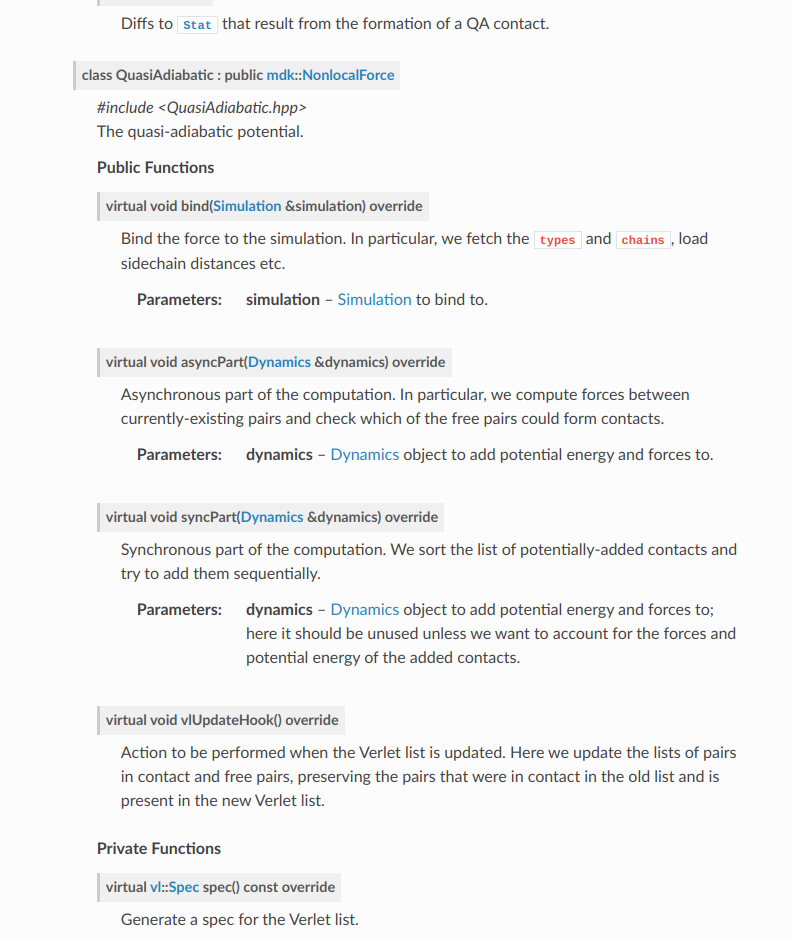
\includegraphics[width = \textwidth]{graphics/docs2.png}
    \caption{Screenshot of the documentation}
    \label{fig:docs}
\end{figure}

Moreover, in order to aid the modification of existing components, inline comments have been provided. However, we have observed that for the most part the documentation of variables in header files and the way the code is structured suffices to explain the semantics of the code, so this part of the documentation was for the most part limited to explaining certain sophisticated optimizations, like the algorithm for the cell-based construction of the Verlet list.
